\section{Rectification}

\begin{frame}
    \begin{itemize}
        \item Ajouter une continuation aux paramètres de la fonction
        \item Remplacer les appels récursifs non terminaux par un appel récursif
              avec une nouvelle continuation
        \item Remplacer les retours de fonction par des appels à la continuation
    \end{itemize}
\end{frame}

\subsection{Ensembles rectifiants}

\begin{frame}[fragile,t]
    \frametitle{Ensembles rectifiants}

    \vspace{-0.2cm}

    \begin{definition}
        Un ensemble de noms de variables $E$ \textit{rectifie} une forme linéaire
        $l$ lorsque tout appel de fonction potentiellement récursif dans $l$
        (directement ou indirectement) est un appel à une fonction dont le nom est
        dans $E$.
    \end{definition}

    \pause

    \small

    \begin{minipage}[t]{0.5\textwidth}
        \small \begin{minted}{ocaml}
let rec sum l =
    match l with
    | [] -> 0
    | x :: q -> x + sum q
        \end{minted}

        \uncover<3->{
            \begin{tikzpicture}[remember picture,overlay]
                \draw[red,thick,rounded corners] ([yshift=13,xshift=130]pic cs:start) rectangle ([yshift=26,xshift=160]pic cs:stop);
            \end{tikzpicture}
            $$E = \{ \texttt{sum} \}$$
        }
    \end{minipage}%
    \begin{minipage}[t]{0.5\textwidth}
        \vspace{-0.8cm}
        \small \begin{align*}
            a_1 :=\  & \texttt{l}                                          \\
            a_2 :=\  & \texttt{match } a_1 \texttt{ with}                  \\
                     & \texttt{| [] -> } \begin{aligned}[t]
                                             a_3 & := 0
                                         \end{aligned}                 \\
                     & \texttt{| x :: q -> } \begin{aligned}[t]
                                                 a_4 & := \texttt{x}           \\
                                                 a_5 & := \texttt{sum}         \\
                                                 a_6 & := \texttt{q}           \\
                                                 a_7 & := a_5 \ a_6            \\
                                                 a_8 & := a_4 \texttt{ + } a_7
                                             \end{aligned}
        \end{align*}

        \uncover<4->{
            \begin{tikzpicture}[remember picture,overlay]
                \draw[red,thick,rounded corners] ([yshift=25,xshift=120]pic cs:start) rectangle ([yshift=38,xshift=145]pic cs:stop);
            \end{tikzpicture}
            \vspace{-0.4cm}
            $$E = \{ \texttt{sum}, a_5 \}$$
        }
    \end{minipage}
\end{frame}

\addtocounter{framenumber}{-1}
\begin{frame}[fragile,t]
    \frametitle{Ensembles rectifiants}

    \begin{minted}{ocaml}
type 'a tree = Leaf of 'a | Node of 'a tree list

let rec visit_children f children =
  match children with
  | [] -> ()
  | x :: q ->
      visit_tree f x;
      visit_children f q

and visit_tree f tree =
  match tree with
  | Leaf value -> f value
  | Node children -> visit_children f children
    \end{minted}

    $$
        E = \{ \texttt{visit\_children}, \texttt{visit\_tree} \}
    $$
\end{frame}

\begin{frame}
    \frametitle{Optimisation des ensembles rectifiants}

    ENS\_RECTIFIANT :
    \vspace{-0.3cm}
    $$
        \left \{ \begin{tabular}{@{}l@{}c@{}l}
            \textbf{Entrée}
             & \textbf{ : }
             & l une forme linéaire, $k \in \mathbb{N}$
            \\ \text{\textbf{Sortie}}
             & \textbf{ : }
             & Existe-t-il un ensemble $E$ rectifiant $l$ tel que $|E| \leq k$?
        \end{tabular} \right .
    $$

    \vspace{0.5cm}
    \pause

    \begin{itemize}
        \item ENS\_RECTIFIANT est \important{indécidable}.
              \pause
        \item Notre algorithme ne marchera pas dans tous les cas possibles.
    \end{itemize}
\end{frame}

\subsection{Rectification}

\begin{frame}[fragile]
    \frametitle{Rectification}

    \RestyleAlgo{plain}
    \small \begin{algorithm}[H]
        \Input{
            Une forme linéaire $l$ ne contenant pas de variables nommées
            \texttt{cont} ou \texttt{new\_cont} et $E$ un ensemble rectifiant $l$.
        }
        \Output{
            Une forme linéaire récursive terminale $l'$ sous CPS équivalente à $l$
        }

        $(a, e) \leftarrow$ le premier élément de $l$ \\
        $q \leftarrow$ le reste de $l$ \\

        \uSi{$e$ contient une définition d'une fonction de $E$}{
            Mettre à jour $e$ tel que la fonction définie dedans:
            \begin{itemize}
                \item Prenne un argument \texttt{cont} en plus
                \item Évalue $Rectifier(l', E)$ lors de son appel o\`u $l'$
                      est la forme linéaire évaluée \\ avant cette redéfinition.
            \end{itemize}
        }

        \uSi{$e$ ne contient pas d'appel à une fonction de $E$}{
            \uSi{$q$ est vide}{
                Renvoyer $\left\{ \hspace{0.2cm} \begin{aligned}
                        a   & := e                & \\
                        res & := \texttt{cont } a &
                    \end{aligned} \right. $
            }
            \strut \ldots
        }
    \end{algorithm}
\end{frame}
\begin{frame}
    \RestyleAlgo{plain}
    \small \begin{algorithm}[H]
        \uSi{$e$ ne contient pas d'appel à une fonction de $E$}{
            \strut \ldots \\
            \uSinon{
                $q_{rec} \leftarrow$ Rectifier($q$, $E$) \\
                Renvoyer $(a, e) \cdot q_{rec}$
            }
        }
        \uSinon{
            \uSi{$e$ est un appel de fonction}{
                $e_{rec} \leftarrow$ $e$ avec \texttt{cont} rajouté en dernier
                argument
            }\uSinon{
                $e_{rec} \leftarrow$ $e$ avec chaque enfant localement terminal $c$
                remplacé par Rectifier($c$, $E$)
            }

            \bigskip

            \uSi{$q$ est vide}{
                Renvoyer $[(a, e_{rec})]$
            }\uSinon{
                $q_{rec} \leftarrow$ Rectifier($q$, $E$) \\
                Renvoyer $\left\{ \hspace{0.2cm} \begin{aligned}
                        \texttt{new\_cont} & := \texttt{fun } a \texttt{ -> } q_{rec} & \\
                        \texttt{cont}      & := \texttt{new\_cont}                    & \\
                        a                  & := e_{rec}                               &
                    \end{aligned} \right.$
            }
        }
    \end{algorithm}
\end{frame}

\begin{frame}
    \frametitle{Correction de Rectifier}

    \begin{proposition}
        Soit $(l, E)$ une entrée de Rectifier. En posant
        $l' = \text{Rectifier}(l, E)$ et $a$ la dernière variable de $l$, pour toute
        fonction $f$, $l.(res, f\ a)$ est équivalent à $(\texttt{cont}, f).l'$.
    \end{proposition}

    \pause

    \begin{proof}
        \begin{enumerate}
            \item On définit Éval($\sigma, l$) et Éval\_opération($\sigma, o$) deux
                  algorithmes mutuellement récursifs.
            \item On procède par récurrence avec:
        \end{enumerate}

        \small
        $$
            P(n): \left \{ \ \parbox{415pt}{$\forall (l, E) \text{ entrée de Rectifier}, \forall \text{fonction } f, \forall \text{environnement } \sigma, \\
                    \text{Éval}(l.[(res, f\ a)], \sigma) \text{ effectue } n \text{ appels à Éval\_opération au total} \implies \\
                    \text{Éval}(l.[(res, f\ a)], \sigma) \text{ a le même résultat que } \\
                    \text{Éval}([(\texttt{cont}, f)].\text{Rectifier}(l, E), \sigma)$} \right .
        $$
    \end{proof}

\end{frame}

\begin{frame}[fragile]
    \frametitle{Application}

    \begin{adjustwidth}{-1.5em}{-1.5em}

        \small \begin{minted}{ocaml}
let rec sum (l : int list) : int =
    match l with
    | [] -> 0
    | x :: q -> x + sum q
        \end{minted}

        \vspace{0.2cm}
        \begin{center}
            $\Big\downarrow$
        \end{center}
        \vspace{0.2cm}

        \small \begin{minted}{ocaml}
let rec sum (l : int list) (cont : int -> 'ret) : 'ret =
    match l with
    | [] -> cont 0
    | x :: q ->
        let new_cont (a_7 : int) : 'ret = cont (x + a_7) in
        sum q new_cont

let s = sum [0; 1; 2] (fun res -> res)
        \end{minted}

    \end{adjustwidth}
\end{frame}

\subsection{Accumulateurs}

\begin{frame}[t]
    \frametitle{Accumulateurs}

    \begin{center}
        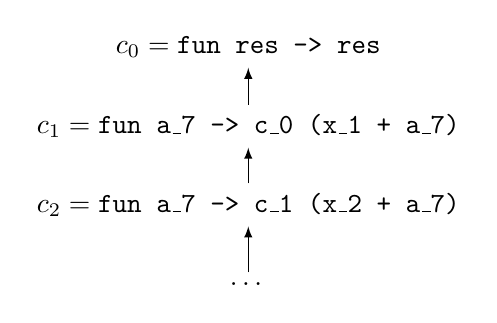
\begin{tikzpicture}
            \node<1-> (c0) at (0, 0) {$c_0 = \texttt{fun res -> res}$};

            \node<2-> (c1) at (0, -1) {$c_1 = \texttt{fun a\_7 -> c\_0 (x\_1 + a\_7)}$};
            \draw<2->[-latex] (c1.north) to (c0.south);

            \node<3-> (c2) at (0, -2) {$c_2 = \texttt{fun a\_7 -> c\_1 (x\_2 + a\_7)}$};
            \draw<3->[-latex] (c2.north) to (c1.south);

            \node<4-> (c3) at (0, -3) {\ldots};
            \draw<4->[-latex] (c3.north) to (c2.south);
        \end{tikzpicture}
    \end{center}
\end{frame}

\addtocounter{framenumber}{-1}
\begin{frame}[t]
    \frametitle{Accumulateurs}

    \begin{center}
        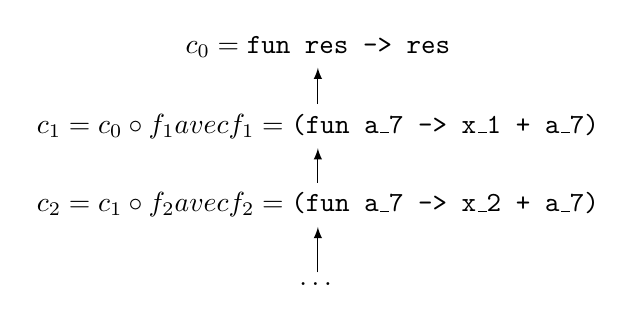
\begin{tikzpicture}
            \node (c0) at (0, 0) {$c_0 = \texttt{fun res -> res}$};

            \node (c1) at (0, -1) {$c_1 = c_0 \circ f_1 \text{ avec } f_1 = \texttt{(fun a\_7 -> x\_1 + a\_7)}$};
            \draw[-latex] (c1.north) to (c0.south);

            \node (c2) at (0, -2) {$c_2 = c_1 \circ f_2 \text{ avec } f_2 = \texttt{(fun a\_7 -> x\_2 + a\_7)}$};
            \draw[-latex] (c2.north) to (c1.south);

            \node (c3) at (0, -3) {\ldots};
            \draw[-latex] (c3.north) to (c2.south);
        \end{tikzpicture}

        \vspace{0.5cm}

        \only<2>{
            $c_n = c_0 \circ f_1 \circ \ldots \circ f_n$
        }
        \only<3>{
            $c_n = f_1 \circ \ldots \circ f_n$
        }
        \only<4>{
            $c_n = f_1 \circ \ldots \circ f_n$
            \par
            $s = f_1(f_2(... f_n(0)))$
        }
        \only<5>{
            $c_n = f_n \circ \ldots \circ f_1$
            \par
            $s = f_n(f_{n-1}(... f_1(0)))$
        }
        \only<6>{
            $c_n = f_n \circ \ldots \circ f_1$
            \par
            $s = f_n(f_{n-1}(... f_1(0)))$

            \begin{itemize}
                \item Chaque continuation est une composition avec la
                      continuation précédente
                \item Les fonctions composées commutent
            \end{itemize}
        }

    \end{center}
\end{frame}

\begin{frame}[fragile]
    \frametitle{Accumulateurs}

    \begin{adjustwidth}{-1.5em}{-1.5em}

        \small \begin{minted}{ocaml}
let rec sum (l : int list) : int =
    match l with
    | [] -> 0
    | x :: q -> x + sum q
        \end{minted}

        \vspace{0.2cm}
        \begin{center}
            $\Big\downarrow$
        \end{center}
        \vspace{0.2cm}

        \small \begin{minted}{ocaml}
let rec sum (l : int list) (acc : int) : int =
  match l with
  | [] -> acc
  | x :: q ->
      let new_acc (a_7 : int) : int = x + a_7 in
      sum q (new_acc acc)

let s = sum [0; 1; 2] 0
        \end{minted}

    \end{adjustwidth}
\end{frame}